\documentclass{book}
\usepackage[english]{babel}
%\usepackage{bookman}
%\usepackage{kmath,kerkis}

\usepackage[T1]{fontenc}
\usepackage[utf8]{inputenc}

\usepackage{graphicx,tikz,wrapfig,hyperref,fancybox,cite}
\usepackage{amsmath,amssymb,amsthm}

\hypersetup{colorlinks}

\renewcommand{\(}{\begin{columns}}
\renewcommand{\)}{\end{columns}}
\newcommand{\<}[1]{\begin{column}{#1}}
\renewcommand{\>}{\end{column}}
\newcommand{\lien}[2]{\mathcal{L}_{#1}^{#2}}
\newcommand{\lie}[1]{\mathcal{L}_{#1}}
\newcommand{\colv}[2]{\begin{pmatrix}#1\\#2\end{pmatrix}}
\newcommand{\bb}[1]{\textbf{#1}}
\newcommand{\mb}[1]{\mathbf{#1}}
\newcommand{\para}{\paragraph}


\newtheorem{definition}{Definition}[section]
\newtheorem{claim}{Claim}[section]
\newtheorem{theorem}{Theorem}[section]
\begin{document}
\title{Investigating piecewise smooth dynamical systems}
\author{Debsankha Manik}
\maketitle

\frontmatter
\chapter{Preface}
Piecewise smooth dynamical systems are of particular interest because of their 
ubiquity and plethora of novel behaviours.  There are very elegant existing frameworks
for analyzing different kinds of border collision bifurcations that occur in those systems.
These include the classic work on border collision of equilibria by Feigin, analysis of grazing 
bifurcations using the ZDM formalism developed by ?Nordmark and the impact map 
approach developed by ?Bernardo.  

Using the ZDM formalism, Banerjee and Kundu analyzed the soft impacting oscillator system
and predicted the onset of chaos immediately following the grazing of a limit 
cycle \emph{except} when the ratio of the damped natural frequency of the 
system and the forcing function frequency are in integral or half integral 
ratios.  Experiments have borne out this prediction, except that chaos has 
been observed to vanish in a \emph{small neighbourhood} of those 


\tableofcontents

\mainmatter
\chapter{Introduction}
\section{Overview}
% Piecewise smooth dynamical systems
Theory of dynamical systems enables us to gain valuable insights into many problems.  By using the powerful 
tools it provides, in many cases we can explain how a system will behave 
when the actual equations governing its evolution are too difficult to solve 
analytically.  This approach has been proved time and again to be extremely 
useful in a diverse range of areas: fluid flows, electrical circuits, 
ecological systems etc.  

However, conventional treatments of the subject generally places the demand 
that the systems be describable in terms of \emph{smooth} functions of the 
dynamical variables. There are valid reasons for doing so.  For a system's 
stability analysis, the Jacobian plays a role of paramount importance.  But 
its existence cannot be guaranteed everywhere in the phase space for non 
smooth systems.  

\begin{figure}
\label{fig-bouncing_ball}
\caption{Trajectory of a bouncing ball : a piecewise smooth system}
\begin{center}
\includegraphics[width=0.4\columnwidth]{bounce}
\end{center}
\end{figure}

Unfortunately, many systems we need to deal with regularly are non smooth: 
electrical circuits involving switches, systems exhibiting sliding or 
chattering motion, impacting systems etc.  One subclass of these systems is 
called  \emph{piecewise smooth} systems. The equation governing the evolution 
of these system changes the moment  the system 
co-ordinates cross what is known as a ``switching manifold'', which is a 
surface with 
dimension lower than that of the phase space.  Between any two of those 
switches, the system evolves smoothly. For example, a ball bouncing against 
the floor under the influence of gravity constitutes such a system.  Between 
any two bounces, the height of the ball $h$ is described by $\ddot{h}=-g/m$, 
where $g$ is the acceleration due to gravity and $m$ is the mass of the ball.  
The solution to the equation is a parabola, as depicted in Fig 
\ref{fig-bouncing_ball}, which is of course a smooth function.  But at the 
instance of the bounce, the velocity of the ball changes changes in a 
non-smooth manner.  Despite the simplicity of the system, it shows rich 
dynamical behaviour for certain parameter values\cite{2010arXiv1002.2448O}.  

% Examples

\section{Classification of piecewise smooth systems}
\subsection{Piecewise smooth maps}

\begin{definition}
A map  described by a \emph{finite} set of \emph{smooth} maps:

\begin{equation}
\label{eq-pwmap}
x\mapsto F_i(x,\mu)~~\forall x\in S_i
\end{equation}

is called a piecewise smooth map if:

\begin{enumerate}
\item 
\begin{eqnarray*}
S_i&\in& \mathbf{X}\hspace{2em} \forall i\\
\cup_i S_i&=&\mathbf{X}\\
S_i\cap S_j&=&\emptyset, \hspace{2em} i\ne j
\end{eqnarray*}

\item Each of the functions $F_i$ is smooth in both the state $x$ and the parameter 
$\mu$ throughout $S_i$.  
\end{enumerate}
\end{definition}
\para{Example: Tent map}
\begin{equation}
\label{eq-tent}
x_{n+1}=f_\mu(x_n)=\begin{cases} \mu x_n & \mathrm{for}~~ x_n < \frac{1}{2} \\ \\ \mu (1-x_n) & \mathrm{for}~~ \frac{1}{2} \le x_n \end{cases}
\end{equation}


\begin{figure}[!htp]
\caption{Tent map}
\begin{center}
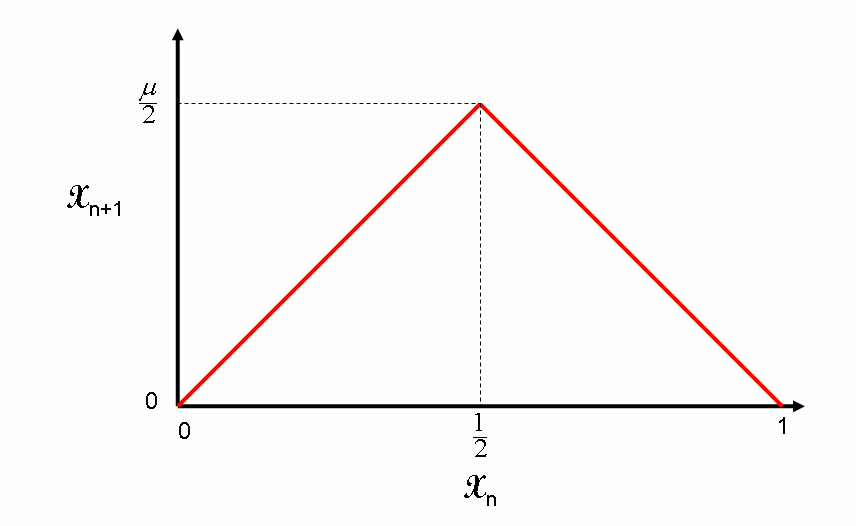
\includegraphics[width=0.7\columnwidth]{Tent_map}
\end{center}
\end{figure}

Now we will define a few quantities to be used extensively in the next 
sections.  

\begin{definition}
\label{def-switching_manifold}
The intersection $\Sigma_{ij}$ between the closures (i.e. the set and its limit points) of 
any pair of $S_i$'s are called the \bb{switching manifolds} of the system:\[
\Sigma_{ij}:=\bar{S_i}\cup\bar{S_j}
\]
\end{definition}
\para{Example:}
In case of the Tent map \eqref{eq-tent}, there is one switching manifold 
$S={1/2}$.  

\begin{definition}
\label{def-sing_order}
For a point $x_0\in\sigma_{ij}$, the leading order term in the power series 
expansion of $F_i(x)-F_j(x)$ about $x_0$ is called the \bb{order of singularity} of the 
map at the point $x_0$.  
\end{definition}
\para{Example:}
In case of tent map, 
\begin{align}
F_2(x)-F_1(x)&=2\mu x-\mu\\
&=0+2\mu(x-\frac{1}{2})
\end{align}
Therefore the order of singularity is $1$. \\


It is obvious that if the map has a \emph{discontinuity} at a point, the order 
of singularity at that point will be $0$. \\ 


We will later see that piecewise smooth maps arise naturally as a result of 
taking Poincáre sections of \emph{piecewise smooth flows} (Something we will 
define right now).

\subsection{Piecewise smooth flows}
Piecewise smooth flows are defined by extending the concept of piecewise smooth maps to 
continuous time systems:
\begin{definition}
A flow  described by a \emph{finite} set of ODE's:

\begin{equation}
\label{eq-pwflow}
\dot{x}=F_i(x,\mu)\hspace{2em}  \forall x\in S_i
\end{equation}

is called a piecewise smooth flow if:

\begin{enumerate}
\item 
\begin{eqnarray*}
S_i&\in& \mathbf{X}\hspace{2em} \forall i\\
\cup_i S_i&=&\mathbf{X}\\
S_i\cap S_j&=&\emptyset, \hspace{2em} i\ne j
\end{eqnarray*}

\item Each of the vector fields $F_i$ is smooth in both the state $x$ and the parameter 
$\mu$ throughout $S_i$.  

\item Each of the vector fields $F_i$  admits a solution $\varphi_i(x)$:
\begin{equation}
\label{eq-def_phi}
\dot{\varphi_i}(x,t)|_{t=0}=F_i(x)~~\forall x\in S_i
\end{equation}

that is smooth in both the state $x$ and the parameter 
$\mu$ throughout $S_i$.  
\end{enumerate}
\end{definition}

\para{Example: Oscillator with soft impacts\\}
\begin{figure}[!hbp]
\caption{Impact oscillator}
\begin{center}
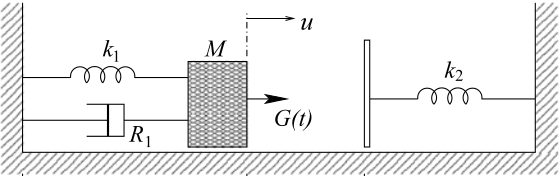
\includegraphics[width=0.5\columnwidth]{osc-pw}
\end{center}
\end{figure}

Consider a simple harmonic oscillator driven by a driving force $G(t)$ which 
hits against another spring attached to the wall at a distance $\sigma$ from 
its equilibrium position. The equation of motion is given by:

\begin{equation}
\label{eq-soft_impact}
m\ddot{x}=
\begin{cases} 
-\gamma \dot{x}-k_1x+G(t)&\mathrm{for}~~x<\sigma
\\ \\ 
-\gamma \dot{x}-k_1x-k_2(x-\sigma)+G(t)&\mathrm{for}~~x\geq\sigma 
\end{cases}
\end{equation}

Switching manifolds of piecewise smooth flows are defined identically to those 
of piecewise smooth maps \eqref{def-switching_manifold}, while order of 
singularities are defined slightly differently:\\

\begin{definition}
For a point $x_0\in\Sigma_{ij}$, the first non zero partial derivative of 
$\varphi_i(x_0,t)-\varphi_j(x_0,t)$ with respect to $t$ at $t=0$ is called the \bb{order of 
singularity} of the 
flow at the point $x_0$.  
\end{definition}

\subsection{Piecewise smooth hybrid systems}
\begin{definition}
A system described by a set of ODE's and a set of \bb{reset maps}:
\begin{align}
\label{}
\label{def-hybrid}
\dot{x}&=F_i(x,\mu),~~\forall x\in S_i\\
s&\mapsto R_{ij}(x,\mu),~~\forall x\in\Sigma_{ij}=\bar{S_i}\cup\bar{S_j}
\end{align}

is called a piecewise smooth hybrid system if all the $R_i$'s, $F_i$'s as well 
as the associated flows $\varphi_i$'s are smooth in both $x$ and the parameter 
$\mu$ in the appropriate regimes.  
\end{definition}

\para{Example: Oscillator with hard impacts\\}
\begin{figure}[!hbp]
\caption{Hard impacting oscillator}
\begin{center}
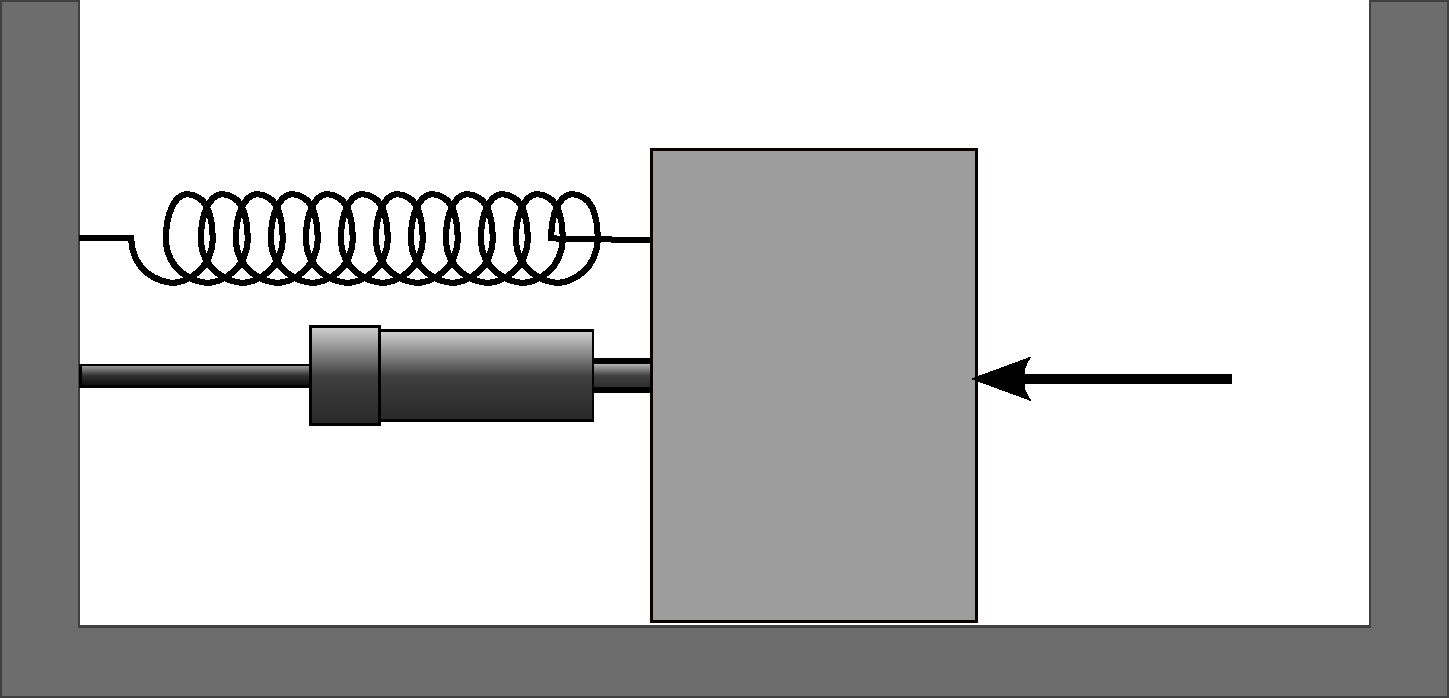
\includegraphics[width=0.5\columnwidth]{hardcol}
\end{center}
\end{figure}

Consider a driven simple harmonic oscillator with a hard wall at a distance 
$\sigma$ from its equilibrium position.   The equation of motion is:
\begin{align}
\label{eq-soft_impact}
m\ddot{x}&=-\gamma \dot{x}-k_1x+G(t)&\mathrm{for}~~x<\sigma\\
(x,v)&\mapsto (x,-rv)&\mathrm{for}~~x=\sigma
\end{align}
Where $r$ is the coefficient of restitution, which is $1$ for perfectly 
elastic collisions.  

% Behaviours specific to it: border collision

\section{Bifurcations in piecewise smooth systems}
Piecewise smooth dynamical systems, quite naturally, can show all the usual 
types of dynamical behaviour shown by smooth dynamical systems : period 
doubling\cite[p.~166-170]{hilborn-chaos} bifurcations, 
saddle-node\cite[p.~109]{hilborn-chaos} bifurcations etc.  \\

However,  piecewise smooth systems exhibit a plethora of interesting behaviours
which involve the sudden change in the system dynamics at the switching 
manifolds and hence, which are not possible in smooth systems. An extensive mathematical 
framework to study these behaviours was first published in the Russian 
literature as early as the seventies of the last century by Mark Feigin\cite{feigin-1970}.
Then these types of behaviours were named \emph{C-bifurcations}.  Now they also go by 
the name of \emph{border collision bifurcations}. We will briefly review a few 
of these novel  behaviours now.   

\begin{figure}[!htp]
\caption{A few cases of border collision bifurcations}
\begin{center}
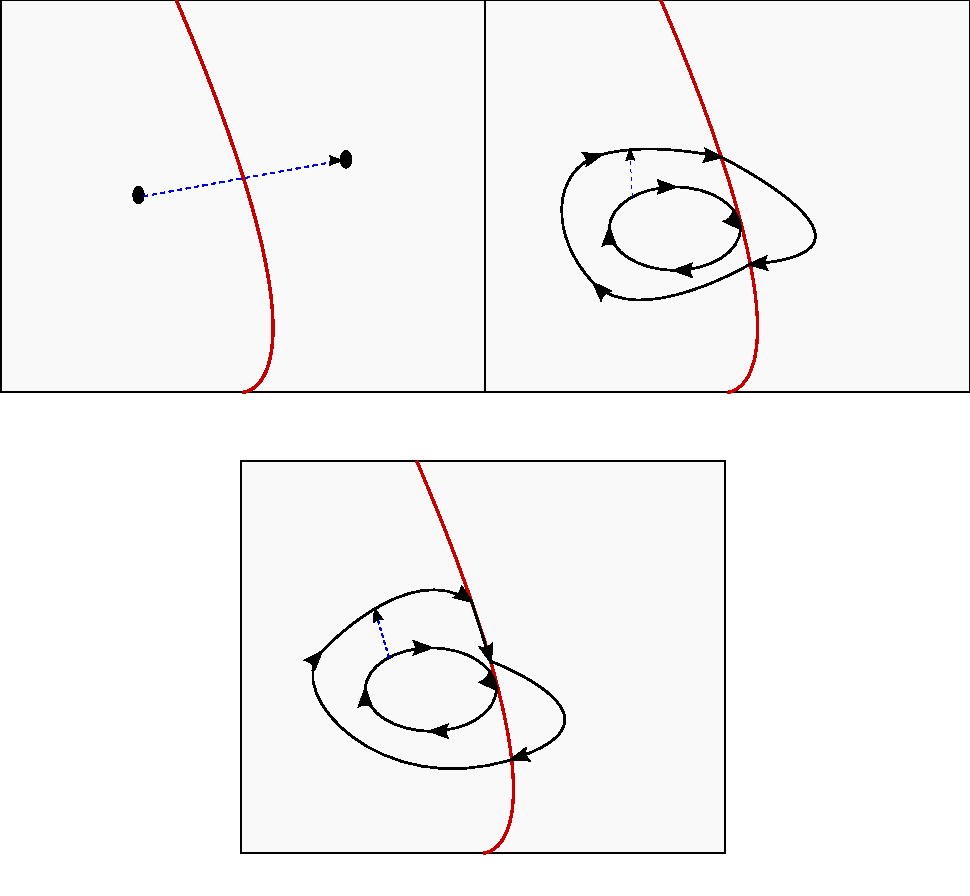
\includegraphics[width=0.9\columnwidth]{c-bifs}
\end{center}
\end{figure}


\subsection{Border collision of equilibria}
Consider a piecewise smooth map:

\begin{equation}
\label{ex-pwflow}
   \dot{\mathbf{x}} = \left\{
     \begin{array}{lr}
       F_1(\mathbf{x}) & : H(\mathbf{x})<0\\
       F_2(\mathbf{x}) & : H(\mathbf{x})>0
     \end{array}
   \right.
\end{equation}

Where $H(x)=0$ defines the switching manifold:
\begin{align*}
S_1&=\left\{x:H(x)<0\right\}\\
S_2&=\left\{x:H(x)\geq0\right\}
\end{align*}

Suppose there exists an equilibrium point of the 
piecewise smooth system $x_1^*(\mu)$ in the region $S_1$ of the phase space:
\[
F_1(x_1^*(\mu))=0
\]


Now, as the parameter $\mu$ is changed, this point will, in general, move in the phase 
space.  Sometimes it may happen that for parameter values $\mu>\mu_0$ this point $s_1^*(\mu)$ crosses the 
boundary and lands up in the region $S_2$.  But in that region $\dot{x}=F_1(x)$ 
is \emph{not the correct ODE in the first place}! Therefore $x_1^*(\mu)$ is no longer 
a fixed point.  We call it a \bb{virtual fixed point}  of the system and such a phenomenon is called 
``border collision of equilibrium''. This phenomenon was first studied by Marc 
Feigin in case of discrete time systems \cite{feigin-1999}(later extended by 
Bernardo \emph{et al} to continuous time systems \cite{bernardo-c-cases}) where he classified the dynamical 
behaviours that can take place when equilibria crosses the switching manifold and 
 derived the necessary conditions for each of them in
terms of the eigenvalues of the Jacobians at both sides of the switching 
manifold. We will now briefly discuss this approach.  

\subsubsection{Types of border collision of equilibria}
Consider a piecewise smooth flow described by \eqref{ex-pwflow}. Let's switch 
to a coordinate system such that the equations of motion look like:

\begin{equation}
\label{ex-pwflow_normal}
   \dot{\mathbf{x}} = \left\{
     \begin{array}{lr}
       F_1(\mathbf{x},\mu) & : x_n<0\\
       F_2(\mathbf{x},\mu) & : x_n\geq0
     \end{array}
   \right.
\end{equation}

(Where $x_n$ denotes the $n$-th component of $\mathbf{x}$.)

Suppose that for every value of the parameter $\mu$, $\exists$ two fixed 
points of the flow, one in each side of the switching manifold:
\begin{align}
\label{def-2fps}
F_1(\mb{x_1^*},\mu)=0,&~~{x_1^*}_n\leq 0\\
F_2(\mb{x_2^*},\mu)=0,&~~{x_2^*}_n\leq 0
\end{align}

We can also assume without loss of generality that the border collision takes 
place for the parameter value $\mu=0$ at the point $\mb{x}=0$:
\[
\mb{x_1^*}=\mb{x_2^*}=\mb{0}~~\text{if } \mu=0
\]


Then we can locally linearize the map:

\begin{displaymath}
   \dot{\bf{x}} = \left\{
     \begin{array}{lr}
       \bf{A_1x+\bf{B}\mu} & : x_n<0\\
       \bf{A_2x+\bf{B}\mu} & : x_n<0\\
     \end{array}
   \right.
\end{displaymath}

Where:\\
\[
\bf{A_i}=\frac{\partial F_1}{\partial \bf{x}}_{x=0}
\]
and 
\[
\bf{B}=\frac{\partial F_1}{\partial \mu}_{\mu=0}=\frac{\partial F_2}{\partial \mu}_{\mu=0}
\]
(Assuming the flow to be continuous at $\mb{x}=0$).

Also, $\bf{A_1}$ and $\bf{A_2}$ can differ only in the $n-$th column (Again 
due to continuity, this time at $\mu=0$).


Now \eqref{def-2fps} becomes:
\begin{align}
A_1\bf{x}^*_1+\bf{B}\mu&=0\\
A_2\bf{x}^*_2+\bf{B}\mu&=0
\end{align}


Assuming $A_i$'s are invertible:

\begin{align}
\label{eq-formula-2fp}
\mb{x}^*_i=-\mb{A_i}^{-1}\mb{B}\mu&=-\frac{adj(\mb{A_i})}{det(\mb{A_i})}\mb{B}\mu
\end{align}
The fixed points $\mb{x^*}_i$ will be real iff
\[
x^*_{1_{n<0}}<0, x^*_{2{_n}}>0. 
\]  

Now, from \eqref{eq-formula-2fp}
\begin{equation}
\label{eq-formula2-2fp}
x^*_{1_k}=\frac{c^*_{1_k}}{det(\bf{A_1})}\mu, x^*_{2_k}=\frac{c^*_{2_k}}{det(\bf{A_2})}
\end{equation}

Where, \[
c^*_{i_k}=[-adj(\bf{A_i)B}]_k
\]

Because $A_1$ differs from $A_2$ only in $n-$th column, $c^*_{1_n}=c^*_{2_n}:=C$

Therefore we have:
\begin{equation}
\label{eq-final-form-2fps}
x^*_{1_n}=\frac{C}{det(\bf{A_1})}\mu, x^*_{2_k}=\frac{C}{det(\bf{A_2})}\mu
\end{equation}

\para{Cases:\\}
\begin{enumerate}
\item $det({\bf A_1})det({\bf A_1})<0$:  $x^*_{1_n}$ and $x^*_{2_n}$ always have 
opposite signs:  In that case, before border collision, there'd be 2 real 
fixed points in opposite sides of the switching manifold. As the parameter is 
changed, they'd \emph{simultaneously} suffer border collision and become 
virtual fixed points.  
\item $det({\bf A_1})det({\bf A_1})>0$:  $x^*_{1_n}$ and $x^*_{2_n}$ always have 
same signs: In that case, initially $\mb{x}_1^*$ will be real and $\mb{x}_2^*$ 
virtual (or vice versa), and after border collision $\mb{x}_1^*$ will become virtual and $\mb{x}_2^*$ 
real.  
\end{enumerate}

\begin{figure}
\caption{Border collision of equilibria}
\begin{center}
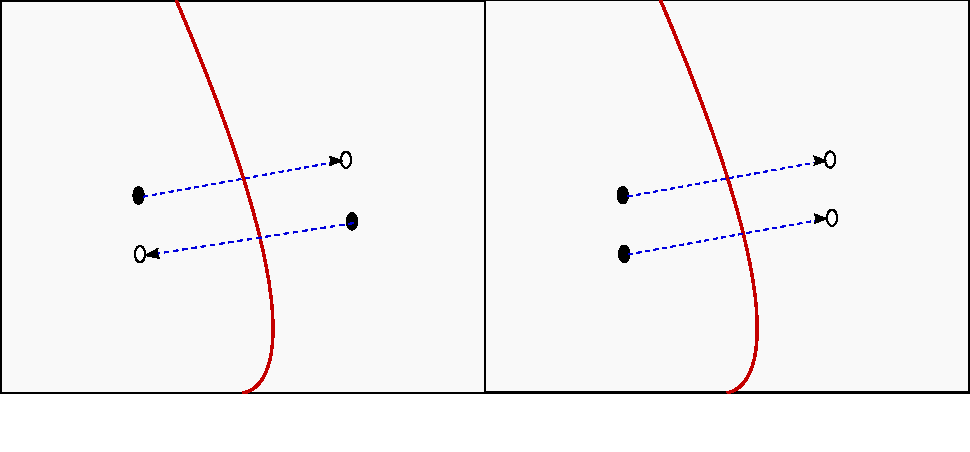
\includegraphics[width=0.9\columnwidth]{cases}
\end{center}
\end{figure}

%\subsubsection{Period doubling at border collision of equilibria}
%Sometimes it may happen that after a fixed point undergoes border collision, a 
%period-2 orbit emerges.  This phenomenon was also studied in great detail by \cite{feigin-1999}.
%Here we discuss in brief a very important necessary condition for this to 
%happen.  
%
%\begin{claim}
%
%Consider a piecewise smooth map of the form \eqref{eq-pwmap}:
%
%\begin{equation}
%x_{n+1}=f(x_n,\mu)=\begin{cases} f_1(x_n,\mu) & \mathrm{for}~~ x_n < 0 \\ \\
%f_2(x_n,\mu)&\mathrm{for}~~ x_n\geq 0 \end{cases}
%\end{equation}
%
%Suppose $\exists$ a fixed point of the map $x_1^*<0$ so long as  the parameter $\mu<0$.  
%Suppose that when $\mu$ equals $0$, $x_1^*$ suffers border collision and on 
%increasing $\mu$ further, a period-2 orbit becomes stable.  Then the Jacobian 
%of the map must suffer a discontinuity at $0$, the point of border collision 
%at the parameter value $\mu=0$
%\end{claim}
%
%\begin{figure}
%\caption{Before border collision: period 1}
%\begin{center}
%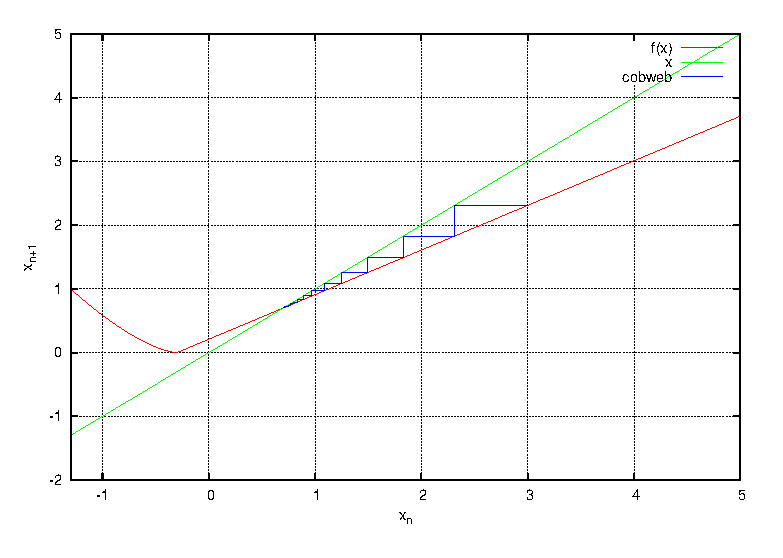
\includegraphics[width=0.7\columnwidth]{pw-perdoub-bef}
%\end{center}
%\end{figure}
%
%\begin{figure}
%\caption{After border collision: period 2}
%\begin{center}
%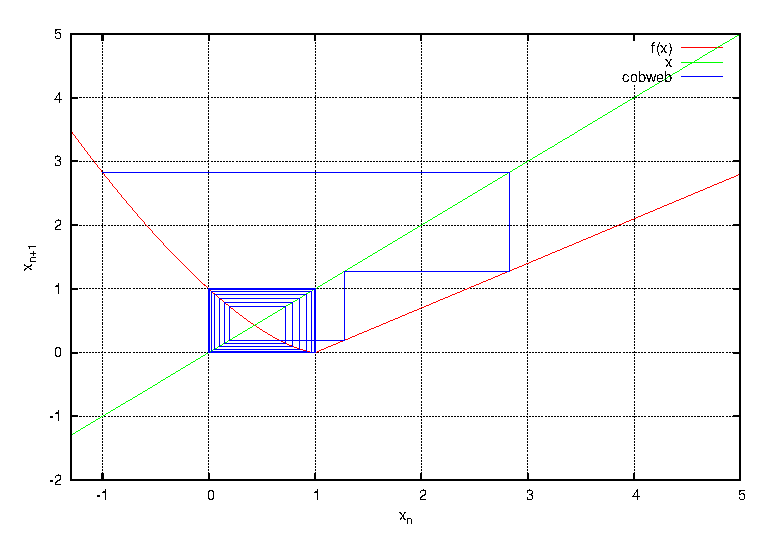
\includegraphics[width=0.7\columnwidth]{pw-perdoub-after}
%\end{center}
%\end{figure}
%


\subsection{Grazing bifurcation of limit cycles due to border collision}

% Order of discontinuity: trace and Jacobian
% ZDM approach
% Chaos narrow band vanishing for integer n : hole: no chaos unexplained
% Impact map.  Budd et al: hole: no damping
% Numerical computation of fixed pt and jacobian 
% Transient lifetimes : unexplored


\chapter{Our system}
% description
% solution x_h and x_p
% approx poincare map
% impact map
% plot of numerical poincare map
% long transients
% hypothesis
% jacobians crossing 1
% FP losing stability?












\bibliography{citations}{}
\bibliographystyle{plain}
\end{document}
